

\section{Webanwendung-GUI Gestaltung} 

Die Abbildung 5.4 veranschaulicht die Startseite der Webanwendung.
Hier werden alle Patienten in einer Liste dargestellt.
Diese Liste ist in die folgenden f\"unf Spalten aufgeteilt.

 \begin{itemize}
  \item Patient:\\
  Hier steht der Name des Patienten.
  
  \item Kalorienzunahme:\\
  In dieser Spalte wird die Menge der Kilokalorien angezeigt, 
  welche der Patient am aktuellen Tag bereits eingenommen hat.
  Ist der Hintergrund \emph{gr\"un}, so ist die eingenommene Menge unterhalb des 
  vorgegebenen Limits.
  Beim \"Uberschreiten der erlaubten Menge wird der Hintergrund \emph{rot} angezeigt.
  
  \item RR/HF:\\
  Hier wird der Blutdruck als Durchschnittswert der letzten vier Tage angezeigt.
  Je nach Klassifikation wird der Hintergrund \emph{gr\"un}, \emph{gelb} oder \emph{rot} 
  gef\"arbt. 
  Die Klassifikation der Blutdruckbereiche richtet sich nach der 
  Weltgesundheitsorganisation (WHO)\cite{WHO:01} und wurde so in die Software \"ubernommen:
  
  \subitem Optimaler Blutdruck: systolisch < 120, diastolisch < 80.
  \subitem Normaler Blutdruck: systolisch < 130, diastolisch < 85.
  \subitem Hochnormaler Blutdruck: systolisch < 140, diastolisch < 90.
  \subitem Hypertonie Grad 1: systolisch < 160, diastolisch < 100.
  \subitem Hypertonie Grad 2: systolisch < 180, diastolisch < 110.
  \subitem Hypertonie Grad 3: systolisch > 179, diastolisch > 109.
  \subitem Isolierte systolische Hypertonie: systolisch > 140, diastolisch < 90.
  
  \item Gewicht:\\
  An dieser Stelle wird das zuletzt gemessene K\"orpergewicht des Patienten angezeigt.
  Der Hintergrund wird je nach Abweichung vom Wunschgewicht in unterschiedlichen 
  F\"arbungen dargestellt:
  \subitem Gr\"un: Abweichung < 10\%.
  \subitem Gelb: Abweichung > 10\%.
  \subitem weiches Rot: Abweichung > 20\%.
  \subitem dunkles Rot: Abweichung > 30\%.
  \subitem grelles Rot: Abweichung > 50\%.
  
  \item Auswahl:\\
  In dieser Spalte befindet sich ein Button, mit dem ein Patient ausgew\"ahlt wird.
  Nach dem Dr\"ucken wird im Bereich \emph{p1} eine Patientenvorschau eingeblendet.
 \end{itemize}

  

\begin{figure}[h]
\centering
  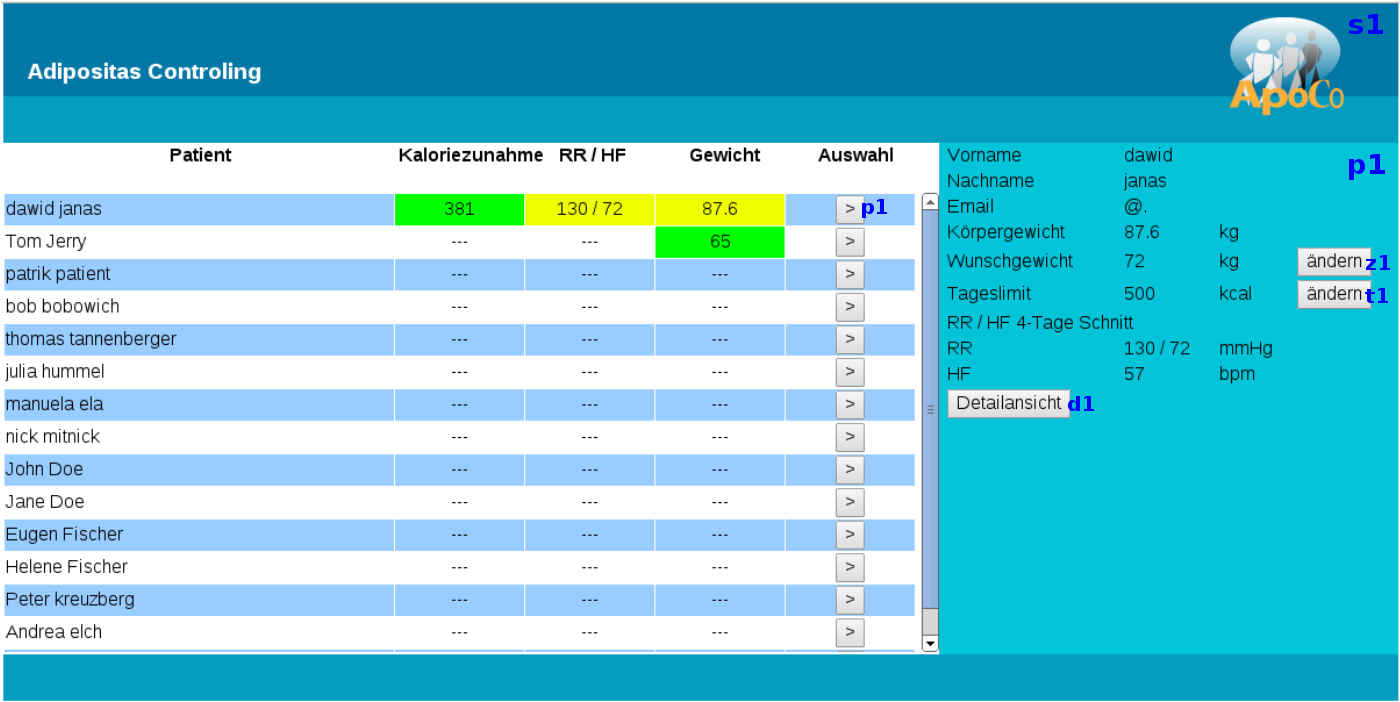
\includegraphics[scale=0.25]{screenshots/kapitel5/startseite_webui_.png}
  \caption{Startseite der Webanwendung}
\end{figure}

In der Vorschau \emph{p1} sind detailierte Informationen zum Patienten und drei weitere 
Buttons enthalten. 
Der Button mit der Bezeichnung \emph{\"andern} und mit der Verlinkung auf \emph{z1}, 
\"offnet einen modalen Dialog zum \"Andern des gew\"unschten K\"orpergewichts 
f\"ur den Patienten.
Der zweite Button mit der Bezeichnung \emph{\"andern} und der Verlinkung auf \emph{t1}, 
\"offnet hingegen einen modalen Dialog zum \"Andern der maximal erlaubten 
\"Kilokalorienmenge f\"ur den Patienten.
Beide Dialoge sind immer aus dem Bereich \emph{p1} erreichbar, wenn dieser eingeblendet ist.
In der Abbildung 5.5 werden beide Dialoge veranschaulicht.\\

\begin{figure}[h]
\centering
  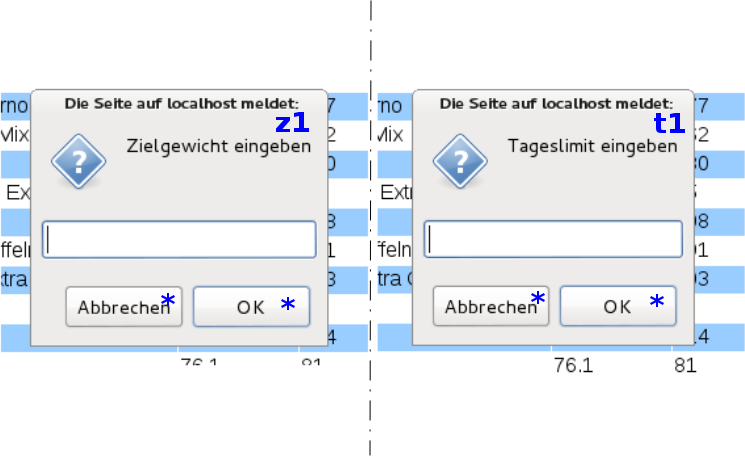
\includegraphics[scale=0.5]{screenshots/kapitel5/modaldialogs_.png}
  \caption{modale Dialoge zum \"Andern vom Zielgewicht und Tageslimit f\"ur einen Patienten}
\end{figure}

In der Abbildung 5.6 und 5.7 wird die Webanwendungsview \emph{d1} dargestellt.
Hier gelangt der Anwender beim Dr\"ucken des Buttons \emph{Detailansicht}.
In dieser View wird im Bereich \emph{p1} zus\"atzlich ein Kalender-Widget eingeblendet.
Im Container \emph{draw-holder} werden Messwerte eines Patienten als Graph \emph{g1}
oder Liste \emph{m1} von protokollierten Mahlzeiten abgebildet.
Das Kalender-Widget dient hier als Steuerelement f\"ur die abgebildeten Werte.
Der Kalender und die Buttons in der \emph{head-navigation} mit der Verlinkung 
auf \emph{ca/g1/m1},
nehmen Einfluss auf den Zeitraum, f\"ur welchen die Daten angezeigt werden sollen.\\

\begin{figure}[h]
\centering
  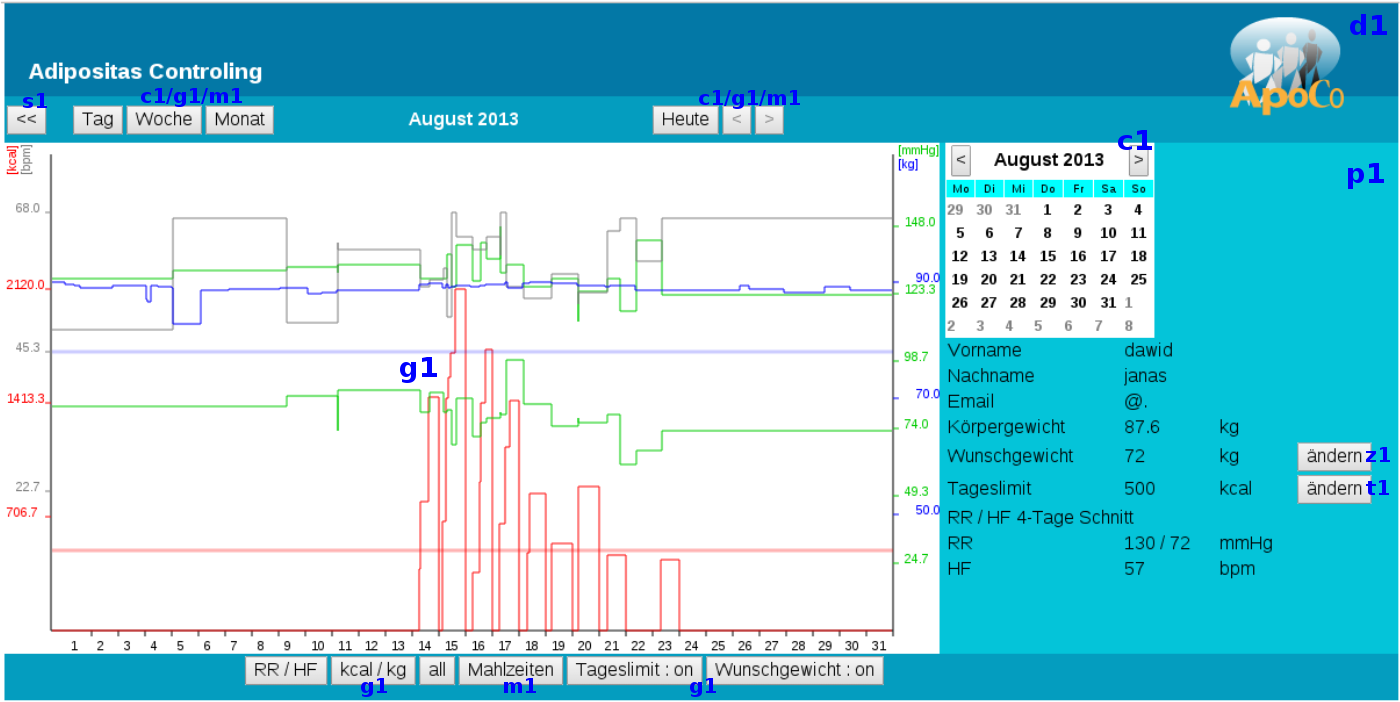
\includegraphics[scale=0.25]{screenshots/kapitel5/patient_graph_.png}
  \caption{Tagesprotokolle in der Graphansicht}
\end{figure}

\begin{figure}[h]
\centering
  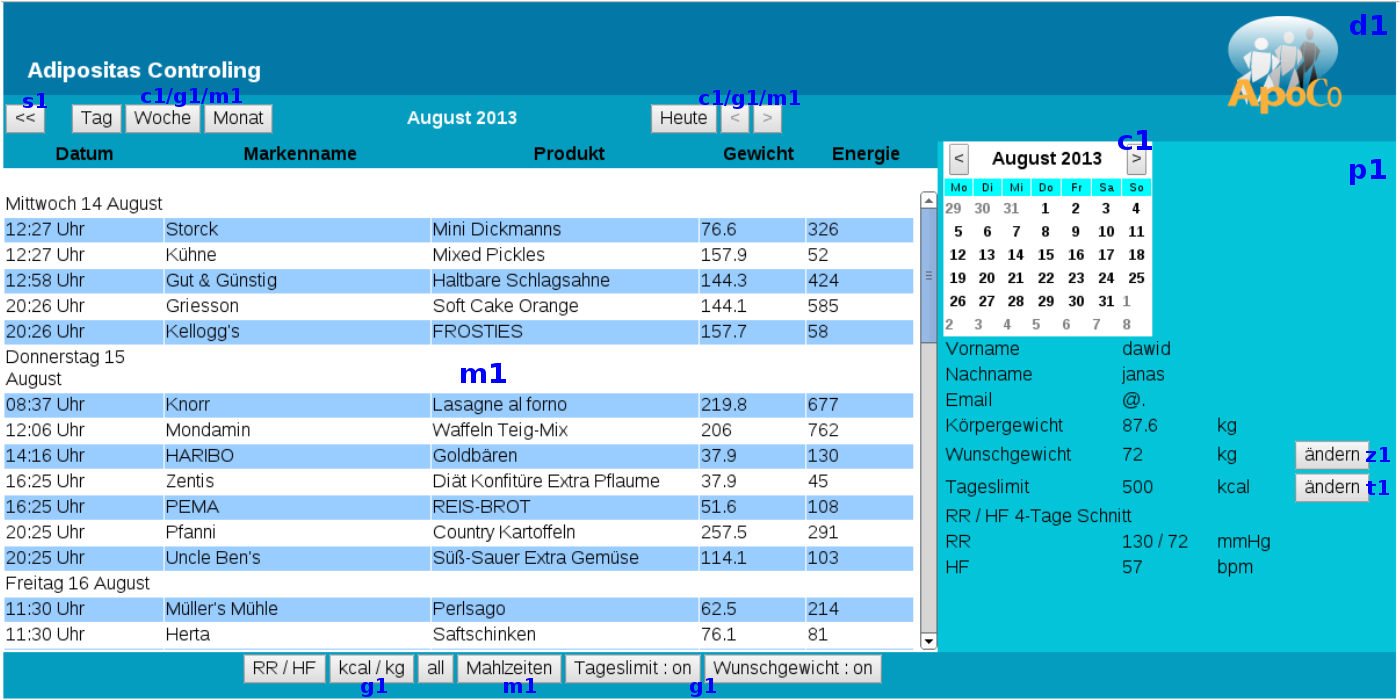
\includegraphics[scale=0.25]{screenshots/kapitel5/meal_list_.png}
  \caption{Mahlzeitenprotokoll}
\end{figure}

Die Abbildung 5.8 pr\"asentiert ein Zustandsdiagramm der Websoftware.
Es verdeutlicht die Beziehungen von Webelementen in der Anwendung untereinander.
Die Modellierung entspricht dem Zustandsdiagramm aus Kapitel 4 in der Abbildung 4.21.
Die Zust\"ande \emph{s1, z1, t1} und \emph{d1} sind mehr globale Zust\"ande der Anwendung.
Sie repr\"asentieren jeweils eine Art View.
Ist die Anwendung im Zustand \emph{d1}, so beinhaltet sie ein Webelement mit zwei 
eigenen Zust\"anden \emph{g1} und \emph{m1}.
Diese repr\"asentieren den Inhalt des Containers \emph{draw-holder}.
Im Zustand \emph{g1} wird ein Graph gezeichnet und im Zustand \emph{m1} eine Liste.\\



\begin{figure}[h]
\centering
  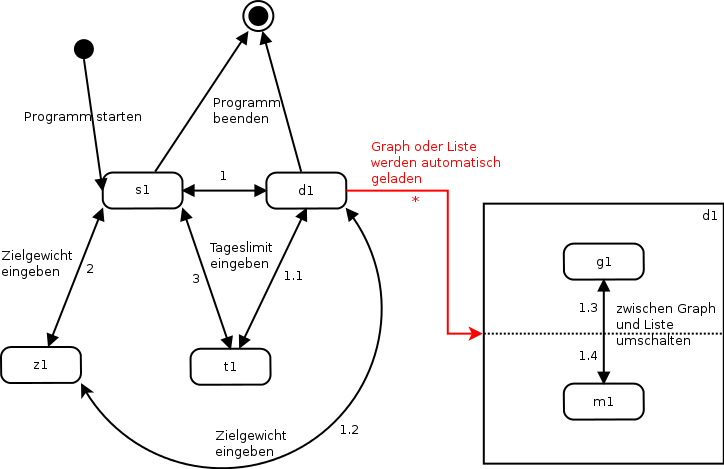
\includegraphics[scale=0.55]{diagramme/kapitel5/zustand_dialog_beziehung_web.png}
  \caption{Zustandsdiagramm der Websoftware}
\end{figure}